\chapter{Dữ liệu và phương pháp đề xuất}

\section{Nguồn dữ liệu}
Dữ liệu được sử dụng trong bài này gồm:
\begin{itemize}[leftmargin=1.5em]
    \item \texttt{Lab\_03/data/pima-indians-diabetes.csv}
    \item \texttt{Lab\_03/data/pima-indians-diabetes.names}
\end{itemize}
Theo file mô tả, bộ dữ liệu có 768 quan sát, 8 thuộc tính số học và 1 biến mục tiêu \texttt{outcome}.

\section{Mô tả thuộc tính}
\begin{table}[H]
\centering
\caption{Mô tả các thuộc tính trong bộ dữ liệu Pima}
\label{tab:pima_features}
\begin{tabular}{p{3.5cm}p{9cm}}
\toprule
\textbf{Thuộc tính} & \textbf{Ý nghĩa}\\
\midrule
pregnancies & Số lần mang thai\\
glucose & Nồng độ glucose huyết tương (2h OGTT)\\
blood\_pressure & Huyết áp tâm trương (mm Hg)\\
skin\_thickness & Độ dày nếp da cơ tay sau (mm)\\
insulin & Nồng độ insulin huyết thanh (2h)\\
bmi & Chỉ số khối cơ thể\\
diabetes\_pedigree\_function & Hệ số tiền sử gia đình\\
age & Tuổi\\
outcome & Nhãn phân lớp (0/1)\\
\bottomrule
\end{tabular}
\end{table}

\section{Kiểm tra chất lượng dữ liệu}
Kết quả từ notebook cho thấy:
\begin{itemize}[leftmargin=1.5em]
    \item Số dòng trùng lặp: 0.
    \item Không có NaN tường minh trong CSV gốc, nhưng có nhiều giá trị \texttt{0} bất thường sinh lý.
    \item Các cột có tỷ lệ \texttt{0} cao: \texttt{insulin} và \texttt{skin\_thickness}.
\end{itemize}

\begin{figure}[H]
\centering
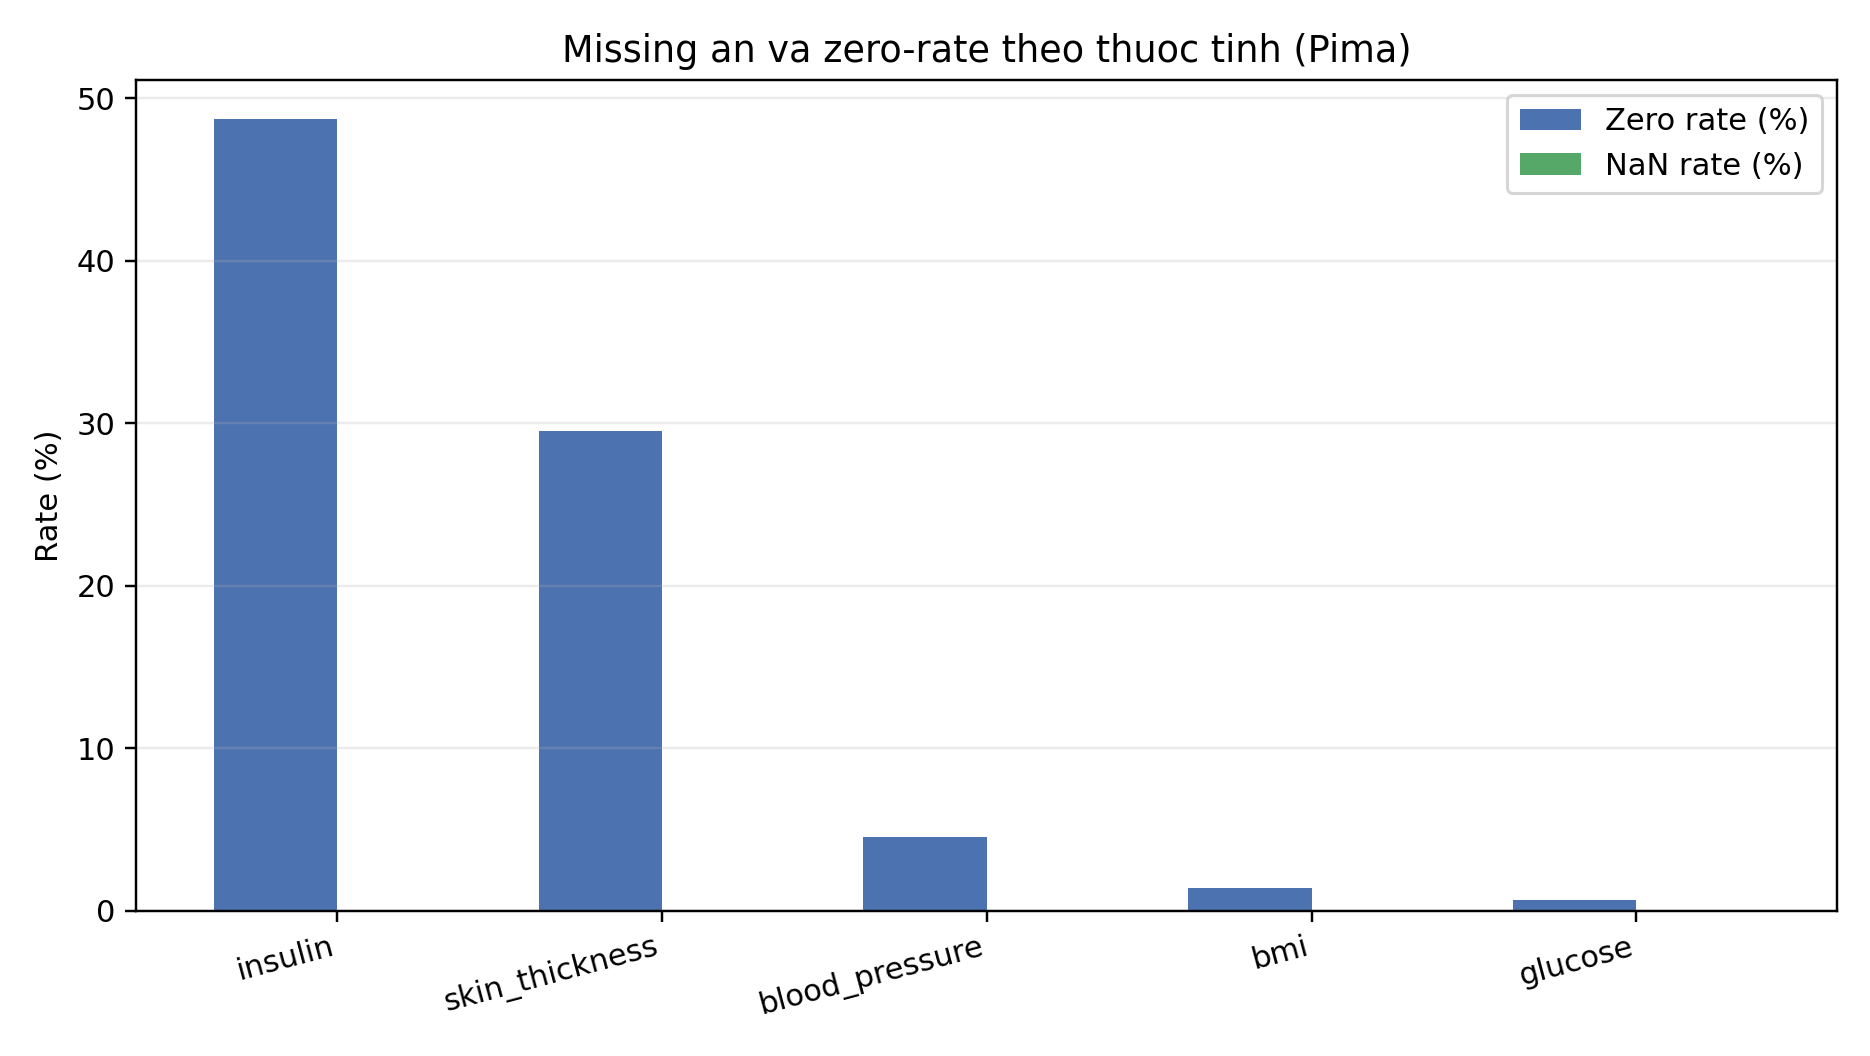
\includegraphics[width=0.82\linewidth]{figures/fig_missing_zero_report.png}
\caption{Thống kê missing ẩn và giá trị 0 theo thuộc tính}
\label{fig:missing_zero_report}
\end{figure}

\section{Quy trình tiền xử lý đề xuất}
Quy trình được đề xuất và triển khai trong notebook:
\begin{enumerate}[leftmargin=1.8em]
    \item Chuyển \texttt{0 -> NaN} cho các biến sinh lý bất thường.
    \item Chia dữ liệu theo tỉ lệ train/validation/test = 60/20/20 (stratified).
    \item Tạo pipeline kết hợp \textit{imputer + scaler + model}.
    \item So sánh 12 tổ hợp cấu hình (3 imputer x 2 scaler x 2 model).
\end{enumerate}

\begin{figure}[H]
\centering
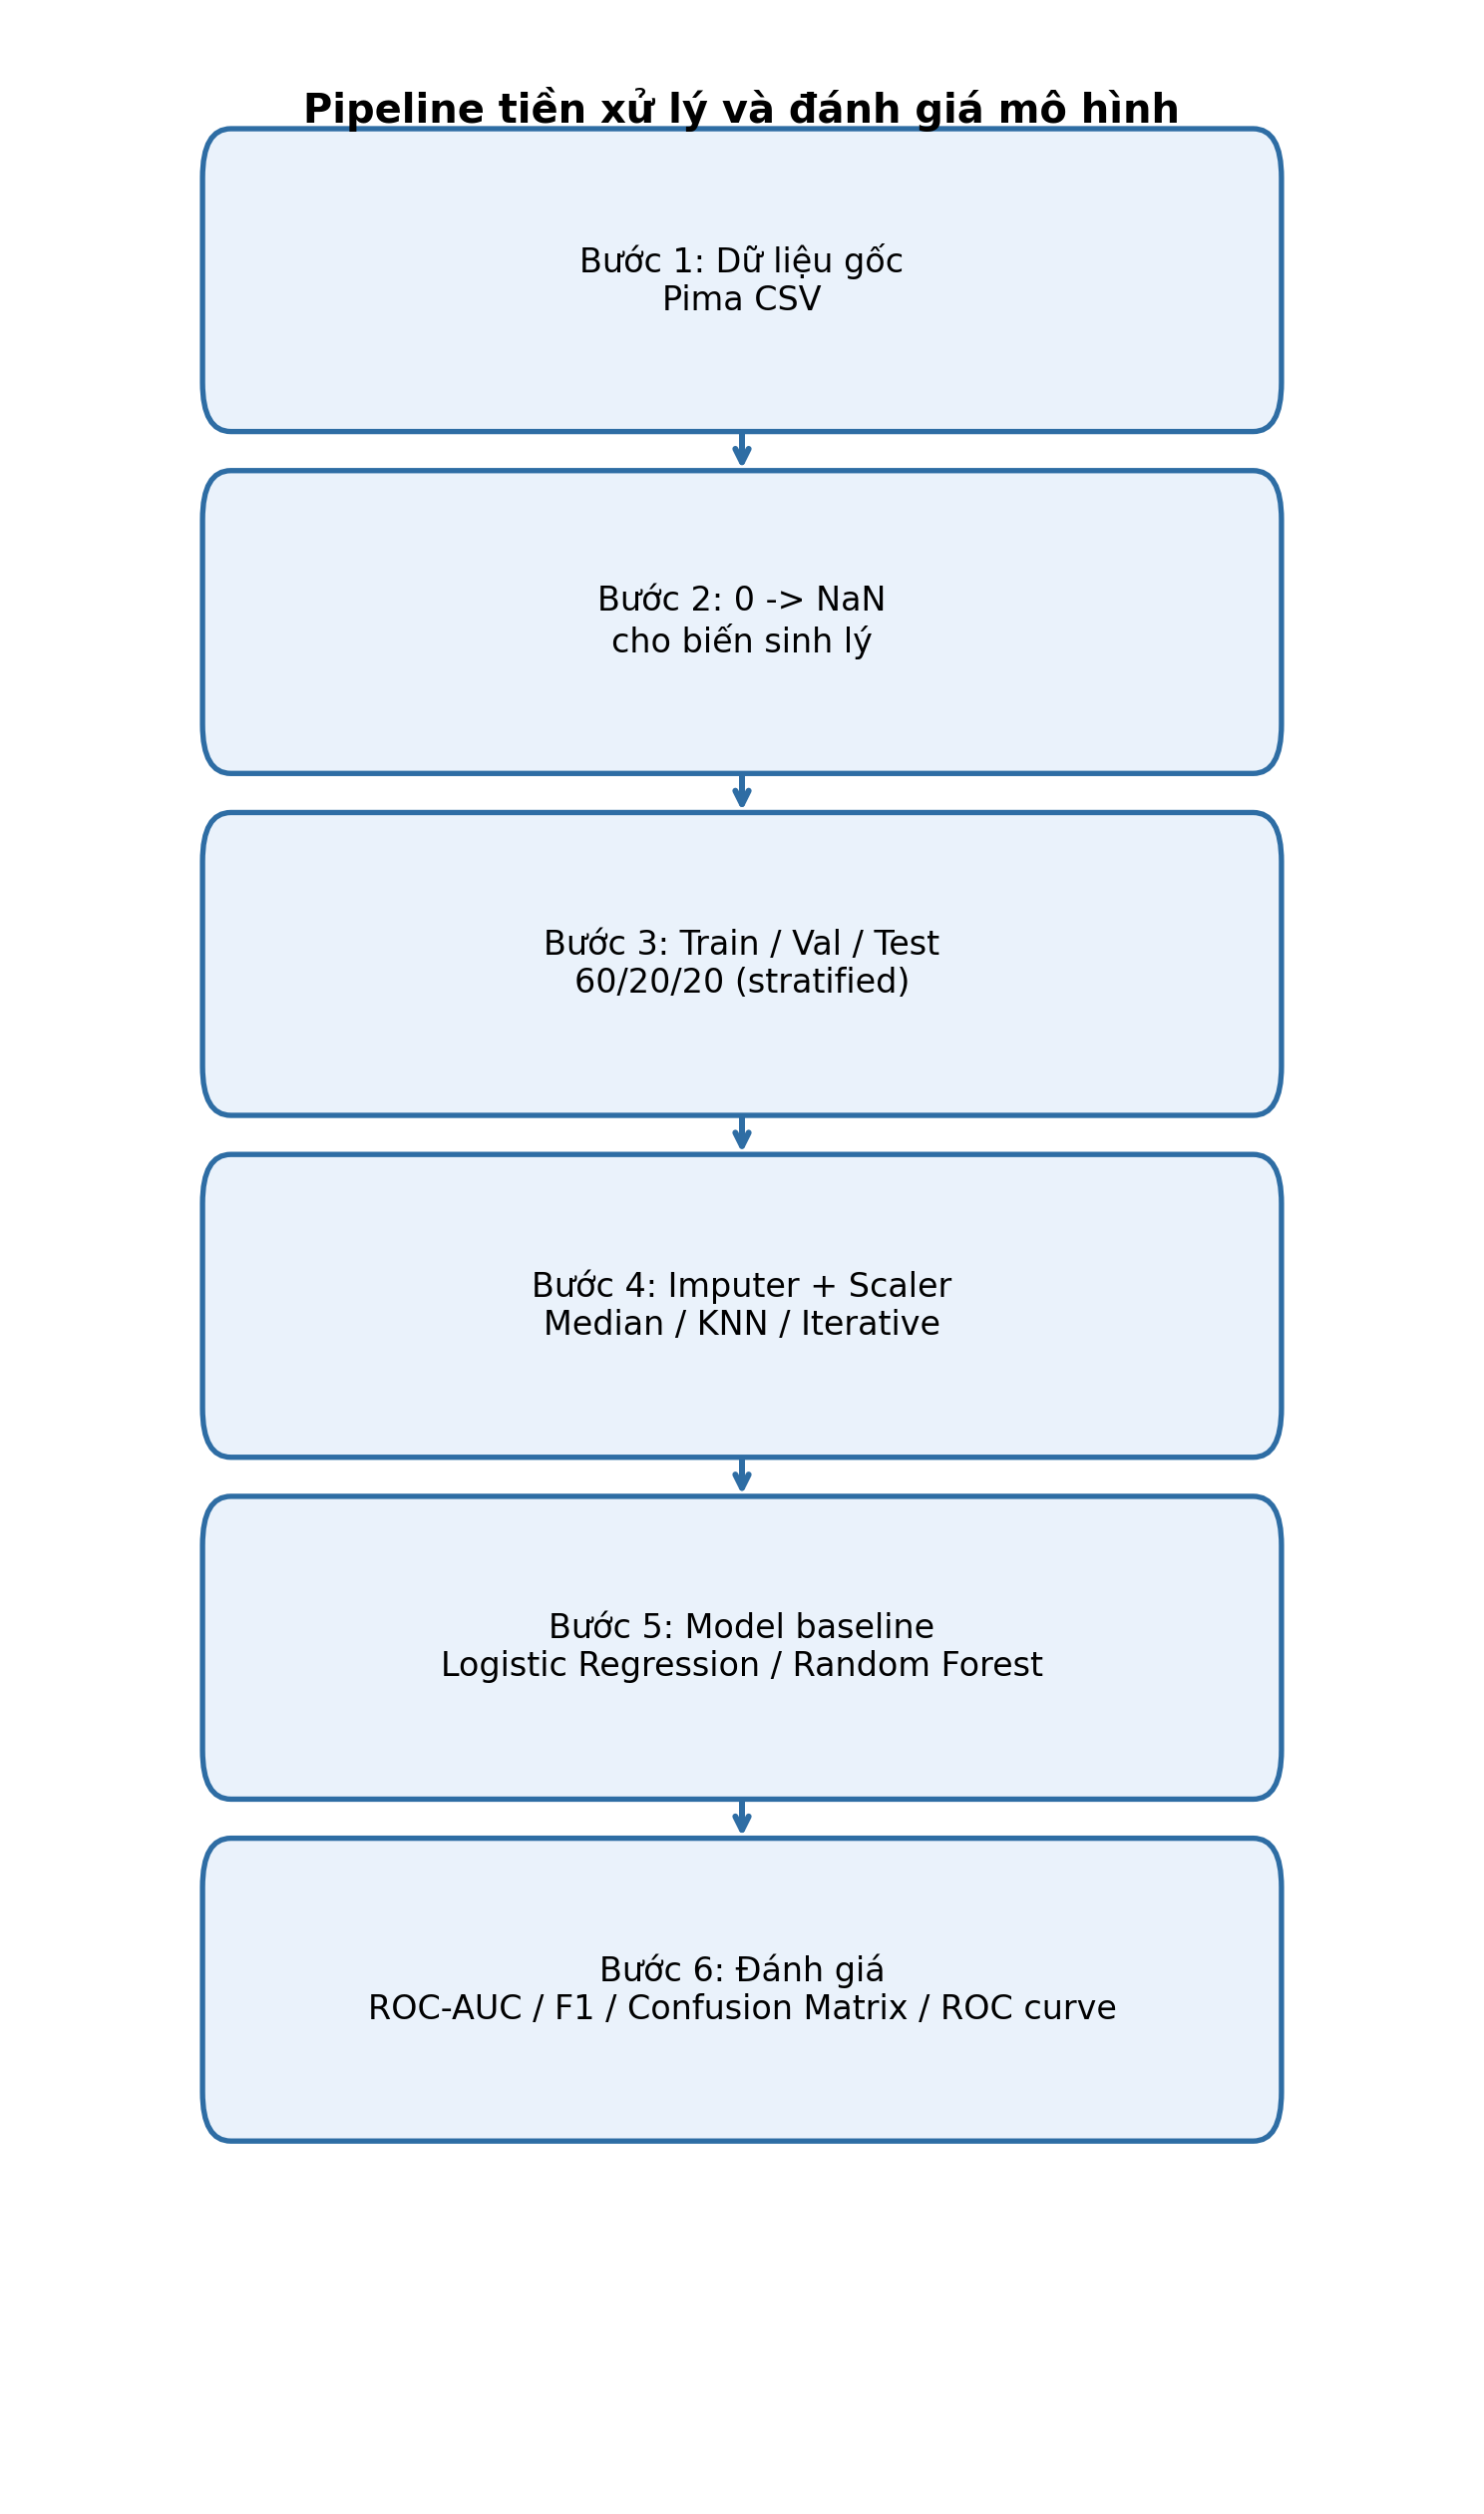
\includegraphics[width=0.62\linewidth]{figures/fig_preprocess_pipeline.png}
\caption{Pipeline tiền xử lý và đánh giá mô hình}
\label{fig:preprocess_pipeline}
\end{figure}
